\chapter{\IfLanguageName{dutch}{Stand van zaken}{State of the art}}%
\label{ch:stand-van-zaken}

% Tip: Begin elk hoofdstuk met een paragraaf inleiding die beschrijft hoe
% dit hoofdstuk past binnen het geheel van de bachelorproef. Geef in het
% bijzonder aan wat de link is met het vorige en volgende hoofdstuk.

% Pas na deze inleidende paragraaf komt de eerste sectiehoofding.

\section{\IfLanguageName{dutch}{Artificiële Intelligentie}{Artificial Intelligence}}%
\label{sec:artificiële-intelligentie}

Artificiële Intelligentie (AI) is een dynamisch en snel evoluerend vakgebied dat zich richt op het ontwikkelen van systemen die taken kunnen uitvoeren die normaal gesproken menselijke intelligentie vereisen, zoals leren, probleemoplossing en besluitvorming \autocite{SharifaniEtAl2023}.

Het doel is om machines te ontwikkelen die autonoom kunnen functioneren in complexe en dynamische omgevingen \autocite{Kouassi2023}.

AI als vakgebied is al meer dan 65 jaar in ontwikkeling en heeft zich inmiddels diep genesteld in ons dagelijks leven. Het speelt immers een curicale rol in sectoren zoals gezondheidszorg, transport, onderwijs en industrie, en wordt gezien als een belangrijke drijfveer voor sociaaleconomische veranderingen en technologische vooruitgang \autocite{JiangEtAl2022}.

Binnen AI zijn Machine Learning (ML) en Deep Learning (DL) twee van de meest revolutionaire technologieën, die de afgelopen jaren aanzienlijke vooruitgang hebben geboekt \autocite{SharifaniEtAl2023}.

\section{\IfLanguageName{dutch}{Machine Learning}}%
\label{sec:machine-learning}

ML is momenteel de meest dominante vorm van AI. Het is een methode voor data-analyse die het mogelijk maakt om analytische modellen automatisch te bouwen en te verbeteren. Het stelt computers in staat om te leren van ervaring, zonder expliciet te worden geprogrammeerd \autocite{SharifaniEtAl2023}.

ML omvat de volgende technieken, die gecombineerd kunnen worden om nog krachtigere en veelzijdigere AI-systemen te ontwikkelen \autocite{Kouassi2023}. 

Supervised Learning (SL): Hierbij wordt een model getraind met behulp van gelabelde gegevens, waarbij zowel de invoer als de gewenste uitvoer bekend zijn. Het model leert in feite door voorbeelden, vergelijkbaar met een leerling die oefent met vragen en de bijbehorende antwoorden. Het doel is om patronen te herkennen die vervolgens kunnen worden gebruikt om voorspellingen te maken voor nieuwe, onbekende gegevens. Voorbeelden van toepassingen zijn het herkennen van spam en het classificeren van afbeeldingen.
Unsupervised Learning (UL): Deze techniek werkt met ongelabelde data, waarbij het model zelf patronen of structuren moet ontdekken. Dit gebeurt vaak door clustering, waarbij vergelijkbare data automatisch worden gegroepeerd. Een voorbeeld is het segmenteren van klanten op basis van koopgedrag. UL is vooral nuttig wanneer er geen duidelijke labels beschikbaar zijn. 
Reinforcement Learning (RL): RL draait om een model dat leert door interactie met een omgeving. Het model probeert een strategie (beleid) te ontwikkelen die maximale beloningen oplevert. Dit wordt vaak gebruikt in scenario's zoals robotica, gaming en autonome voertuigen, waarbij het model leert door trial-and-error. 


Dit hoofdstuk bevat je literatuurstudie. De inhoud gaat verder op de inleiding, maar zal het onderwerp van de bachelorproef *diepgaand* uitspitten. De bedoeling is dat de lezer na lezing van dit hoofdstuk helemaal op de hoogte is van de huidige stand van zaken (state-of-the-art) in het onderzoeksdomein. Iemand die niet vertrouwd is met het onderwerp, weet nu voldoende om de rest van het verhaal te kunnen volgen, zonder dat die er nog andere informatie moet over opzoeken \autocite{Pollefliet2011}.

Je verwijst bij elke bewering die je doet, vakterm die je introduceert, enz.\ naar je bronnen. In \LaTeX{} kan dat met het commando \texttt{$\backslash${textcite\{\}}} of \texttt{$\backslash${autocite\{\}}}. Als argument van het commando geef je de ``sleutel'' van een ``record'' in een bibliografische databank in het Bib\LaTeX{}-formaat (een tekstbestand). Als je expliciet naar de auteur verwijst in de zin (narratieve referentie), gebruik je \texttt{$\backslash${}textcite\{\}}. Soms is de auteursnaam niet expliciet een onderdeel van de zin, dan gebruik je \texttt{$\backslash${}autocite\{\}} (referentie tussen haakjes). Dit gebruik je bv.~bij een citaat, of om in het bijschrift van een overgenomen afbeelding, broncode, tabel, enz. te verwijzen naar de bron. In de volgende paragraaf een voorbeeld van elk.

\textcite{Knuth1998} schreef een van de standaardwerken over sorteer- en zoekalgoritmen. Experten zijn het erover eens dat cloud computing een interessante opportuniteit vormen, zowel voor gebruikers als voor dienstverleners op vlak van informatietechnologie~\autocite{Creeger2009}.

Let er ook op: het \texttt{cite}-commando voor de punt, dus binnen de zin. Je verwijst meteen naar een bron in de eerste zin die erop gebaseerd is, dus niet pas op het einde van een paragraaf.

\begin{figure}
  \centering
  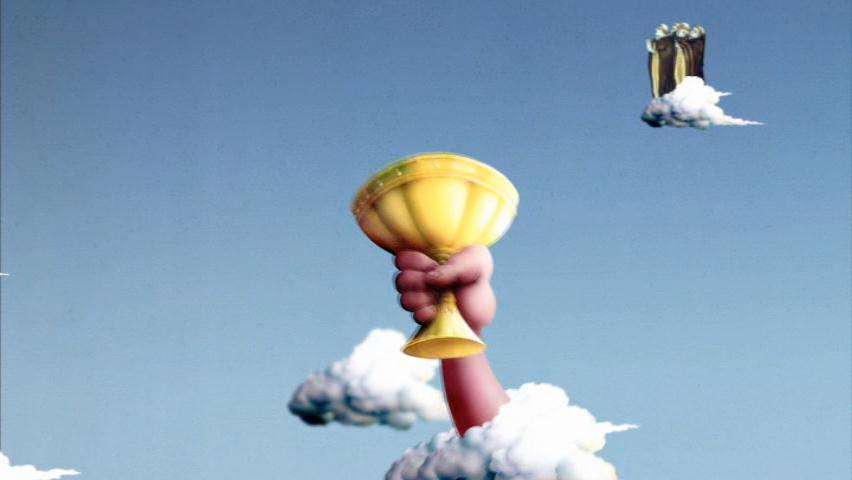
\includegraphics[width=0.8\textwidth]{grail.jpg}
  \caption[Voorbeeld figuur.]{\label{fig:grail}Voorbeeld van invoegen van een figuur. Zorg altijd voor een uitgebreid bijschrift dat de figuur volledig beschrijft zonder in de tekst te moeten gaan zoeken. Vergeet ook je bronvermelding niet!}
\end{figure}

\begin{listing}
  \begin{minted}{python}
    import pandas as pd
    import seaborn as sns

    penguins = sns.load_dataset('penguins')
    sns.relplot(data=penguins, x="flipper_length_mm", y="bill_length_mm", hue="species")
  \end{minted}
  \caption[Voorbeeld codefragment]{Voorbeeld van het invoegen van een codefragment.}
\end{listing}

\lipsum[7-20]

\begin{table}
  \centering
  \begin{tabular}{lcr}
    \toprule
    \textbf{Kolom 1} & \textbf{Kolom 2} & \textbf{Kolom 3} \\
    $\alpha$         & $\beta$          & $\gamma$         \\
    \midrule
    A                & 10.230           & a                \\
    B                & 45.678           & b                \\
    C                & 99.987           & c                \\
    \bottomrule
  \end{tabular}
  \caption[Voorbeeld tabel]{\label{tab:example}Voorbeeld van een tabel.}
\end{table}

